\documentclass{article}

\usepackage[letterpaper,margin=1in]{geometry}
\usepackage{fancyhdr}
\usepackage{marginnote}
\usepackage{amsmath}
\usepackage{amssymb}
\usepackage{tikz}
\usepackage{csquotes}
\usepackage{tabularx}
\usepackage[hidelinks]{hyperref}

\MakeOuterQuote{"}

\colorlet{grx}{green!50!black}

\newcommand{\R}{\mathbb{R}}
\newcommand{\T}{\text{T}}
\newcommand{\dy}{\text{d}y}
\newcommand{\dx}{\text{d}x}
\newcommand{\dd}[2][]{\frac{\text{d}#1}{\text{d}#2}}
\newcommand{\e}{\text{e}}

\newenvironment{tchart}[3]
{
    \renewcommand{\arraystretch}{#1}
    \tabularx{\linewidth}{X|X}
    \multicolumn{1}{c|}{\textbf{#2}} & \multicolumn{1}{c}{\textbf{#3}}\\
    \hline
}{
    \endtabularx
    \renewcommand{\arraystretch}{1}
}

\newenvironment{amatrix}[1]{
    \left[\begin{array}{@{}*{#1}{c}|c@{}}
}{
    \end{array}\right]
}

\renewcommand{\labelitemiii}{\scriptsize$\blacksquare$}

\pagestyle{fancy}
\fancyhf{}
\rfoot{Labalme \thepage}
\rhead{(H) Linear Algebra}

\reversemarginpar

\begin{document}




\lhead{Chapter 6: Eigenvalues}
\section*{Introduction to Eigenvalues and Eigenvectors}
\begin{itemize}
    \item \marginnote{1/28:}[-8.5mm]$Ax=b=\lambda x$
    \item $Ax=\lambda x$, $\lambda\in\mathbb{F}$, $x\in\mathbb{R}^n$
    \item $\lambda$ is an eigenvalue. $\lambda x$ is an eigenvector.
    \begin{equation*}
        A=
        \begin{bmatrix}
            3 & 1\\
            1 & 3\\
        \end{bmatrix}
    \end{equation*}
    \item $
        x =
        \begin{bmatrix}
            1\\
            1\\
        \end{bmatrix}
    $ is an eigenvector of $A$ with corresponding eigenvalue of $4$.
    \item $
        \begin{bmatrix}
            3 & 1\\
            1 & 3\\
        \end{bmatrix}
        \begin{bmatrix}
            1\\
            1\\
        \end{bmatrix}
        =
        \begin{bmatrix}
            4\\
            4\\
        \end{bmatrix}
        = 4
        \begin{bmatrix}
            1\\
            1\\
        \end{bmatrix}
    $
    \begin{center}
        \begin{tikzpicture}
            \draw (-2,0) -- (2,0);
            \draw (0,-2) -- (0,2);
            \draw [thick,->] (0,0) -- node[right]{$x$} (0.5,0.5);
            \draw [thick,dashed,->] (0,0) -- node[right]{$Ax$} (2,2);
        \end{tikzpicture}
    \end{center}
    \begin{align*}
        Ax &= \lambda x\\
        Ax-\lambda x &= 0\\
        Ax-\lambda Ix &= 0\\
        (A-\lambda I)x &= 0
    \end{align*}
    \item $(A-\lambda I)x=0 \Rightarrow x\in N(A-\lambda I)^[$\footnote{To have a null space, $A-\lambda I$ has free columns.}$^] \Rightarrow |A-\lambda I|=0$
    \item $
        \begin{bmatrix}
            3 & 1\\
            1 & 3\\
        \end{bmatrix}
        -
        \begin{bmatrix}
            \lambda & 0\\
            0 & \lambda\\
        \end{bmatrix}
        =
        \begin{bmatrix}
            3-\lambda & 1\\
            1 & 3-\lambda\\
        \end{bmatrix}
    $
    \item $
        \begin{vmatrix}
            3-\lambda & 1\\
            1 & 3-\lambda\\
        \end{vmatrix}
        = 0
    $
    \begin{align*}
        0 &= (3-\lambda)^2-1^2\\
        &= 3^2-6\lambda+\lambda^2-1\\
        &= \lambda^2-6\lambda+8\\
        &= (\lambda-4)(\lambda-2)
    \end{align*}
    \item $\lambda=4,2$.
    \item $\lambda^2-6\lambda+8$ is the \textbf{characteristic polynomial} of $A$.
    \item $
        A-2I =
        \begin{bmatrix}
            -1 & 1\\
            1 & -1\\
        \end{bmatrix}
        ,\ 
        x =
        \begin{bmatrix}
            1\\
            -1\\
        \end{bmatrix}
        \in N(A-2I)
    $.
    \item $
        A-4I =
        \begin{bmatrix}
            -1 & 1\\
            1 & -1\\
        \end{bmatrix}
        ,\ 
        x =
        \begin{bmatrix}
            1\\
            1\\
        \end{bmatrix}
        \in N(A-4I)
    $.
    \item "Eigenspace" is not $\mathbb{R}^2$, but two lines in $\mathbb{R}^2$, specifically $y=\pm x$.
    \begin{itemize}
        \item $y=\pm x$ comes from $c_1\begin{bmatrix}1\\1\end{bmatrix}$ and $c_2\begin{bmatrix}1\\-1\end{bmatrix}$.
    \end{itemize}

    %%%%%%%%%%%%%%%%%%%%%%

    \marginnote{1/29:}\begin{equation*}
        A =
        \begin{bmatrix}
            2 & -2 & 3\\
            0 & 3 & -2\\
            0 & -1 & 2\\
        \end{bmatrix}
    \end{equation*}
    \begin{align*}
        P(\lambda) &= |A-\lambda I|\\
        &=
        \begin{vmatrix}
            2-\lambda & -2 & 3\\
            0 & 3-\lambda & -2\\
            0 & -1 & 2-\lambda\\
        \end{vmatrix}\\
        &= -1
        \begin{vmatrix}
            2-\lambda & 3\\
            0 & -2\\
        \end{vmatrix}
        (-1)^{3+2} + (2-\lambda)
        \begin{vmatrix}
            2-\lambda & -2\\
            0 & 3-\lambda\\
        \end{vmatrix}
        (-1)^{3+3}\\
        &= ((2-\lambda)(-2))+(2-\lambda)((2-\lambda)(3-\lambda))\\
        &= -4+2\lambda+(2-\lambda)^2(3-\lambda)\\
        &= -4+2\lambda+(4-4\lambda+\lambda^2)(3-\lambda)\\
        &= -4+2\lambda+12-4\lambda-12\lambda+4\lambda^2+3\lambda^2-\lambda^3\\
        &= -\lambda^3+7\lambda^2-14\lambda+8\\
        &= -(\lambda-1)(\lambda-2)(\lambda-4)
    \end{align*}
    \begin{align*}
        A-I &=
        \begin{bmatrix}
            1 & -2 & 3\\
            0 & 2 & -2\\
            0 & -1 & 1\\
        \end{bmatrix}&
        A-2I &=
        \begin{bmatrix}
            0 & -2 & 3\\
            0 & 1 & -2\\
            0 & -1 & 0\\
        \end{bmatrix}&
        A-4I &=
        \begin{bmatrix}
            -2 & -2 & 3\\
            0 & -1 & -2\\
            0 & -1 & -2\\
        \end{bmatrix}&
    \end{align*}
    \item $P(\lambda)$ is positive when $n\in 2\mathbb{N}$, negative otherwise.
    \begin{itemize}
        \item Signs flip term to term (think about binomial expansion).
    \end{itemize}
    \item Coefficients of the $n-1$ degree term is the sum of the diagonal entries.
    \item Coefficient of the $0^\text{th}$ degree term is $|A|$.
    \begin{itemize}
        \item $P_\lambda(0) = |A-0\cdot I| = |A|$.
    \end{itemize}
    \item Product of the eigenvalues is $|A|$.
    \begin{itemize}
        \item Think about expanding the factorization.
    \end{itemize}
    \item Eigenvalues of $U$ are the diagonal values.
    \begin{itemize}
        \item $\lambda_1\lambda_2\cdots\lambda_n=|A|$, which is the product of the diagonal entries.
        \item $\lambda_1+\cdots+\lambda_n=\text{trace}(A)$, which is the sum of the diagonal entries.
    \end{itemize}
    \item $Ax=\lambda x$
    \begin{itemize}
        \item $A^2x=AAx=A\lambda x=\lambda Ax=\lambda\lambda x=\lambda^2x$
    \end{itemize}
\end{itemize}



\section*{Similarity}
\begin{itemize}
    \item \marginnote{1/30:}$A\sim B$$^[$\footnote{$A$ "is similar to" $B$}$^]$ iff $\exists\ S:A=SBS^{-1},\ B=S^{-1}AS$.
    \begin{enumerate}
        \item If $A\sim B$, then $|A|=|B|$.
        \begin{align*}
            B &= S^{-1}AS\\
            |B| &= |S^{-1}AS|\\
            |B| &= |S^{-1}||A||S|\\
            |B| &= \frac{1}{|S|}|A||S|\\
            |B| &= |A|
        \end{align*}
        \item If $A\sim B$, then they share the same characteristic polynomial.
        \begin{align*}
            B &= S^{-1}AS\\
            |B-\lambda I| &= |S^{-1}AS-\lambda I|\\
            &= |S^{-1}AS-\lambda S^{-1}IS|\\
            &= |S^{-1}S(A-\lambda I)|\\
            &= |I(A-\lambda I)|\\
            |B-\lambda I| &= |A-\lambda I|
        \end{align*}
        \begin{itemize}
            \item If they have the same characteristic polynomial, $\therefore$ $A$ and $B$ have the same eigenvalues.
        \end{itemize}
    \end{enumerate}
    \item What is the best possible $B$ if $A\sim B$?
    \begin{itemize}
        \item Sparse.
        \item Diagonal.
        \item $
            A=[\text{ugly}]\quad\rightarrow\quad
            B=\begin{bmatrix}
                \lambda_1 &  & 0\\
                 & \ddots & \\
                0 &  & \lambda_n\\
            \end{bmatrix}
            =\Lambda
        $
    \end{itemize}
    \item \textbf{Diagonalization}:
    \begin{align*}
        A &= S\Lambda S^{-1}\\
        AS &= S\Lambda\\
        \Lambda &= S^{-1}AS
    \end{align*}
    \item $A=S\Lambda S^{-1}$
    \begin{itemize}
        \item $A^2 = AA = S\Lambda S^{-1}S\Lambda S^{-1} = S\Lambda\Lambda S^{-1} = S\Lambda^2 S^{-1}$
        \item $A^k = S\Lambda^k S^{-1}$
        \item $
            A^k = S
            \begin{bmatrix}
                {\lambda_1}^k &  & 0\\
                 & \ddots & \\
                0 &  & {\lambda_n}^k\\
            \end{bmatrix}
            S^{-1}
        $
    \end{itemize}
    \item Diagonalize the following matrix $A$.
    \begin{equation*}
        A =
        \begin{bmatrix}
            -1 & 0 & 1\\
            3 & 0 & -3\\
            1 & 0 & -1\\
        \end{bmatrix}
    \end{equation*}
    \begin{itemize}
        \item Find the characteristic polynomial.
        \begin{align*}
            |A-\lambda I| &=
            \begin{vmatrix}
                -1-\lambda & 0 & 1\\
                3 & 0-\lambda & -3\\
                1 & 0 & -1-\lambda\\
            \end{vmatrix}\\
            &= (-1-\lambda)((-\lambda)(-1-\lambda))+(-1)(-\lambda)\\
            &= -\lambda(-1-\lambda)^2+\lambda\\
            &= -\lambda(1+2\lambda+\lambda^2)+\lambda\\
            &= -\lambda^3-2\lambda^2\\
            &= -\lambda^2(\lambda+2)
        \end{align*}
        \item Find the eigenvalues: $\lambda_1=\lambda_2=0$, $\lambda_3=-2$
        \item \textbf{Algebraic multiplicity} of $\lambda_1,\lambda_2$ is 2.
        \item A.M. of $\lambda_3$ is 1.
        \item $
            A-0I =
            \begin{bmatrix}
                -1 & 0 & 1\\
                3 & 0 & -3\\
                1 & 0 & -1\\
            \end{bmatrix}
        $
        \item $\text{rank}(A-0I)=1 \Rightarrow \dim(N(A-0I))=2$
        \item The 2 directly above is the \textbf{geometric multiplicity}.
        \item $A$ is diagonalizable iff A.M. of $\lambda_i=\text{G.M.}$
        
        %%%%%%%%%%%%%%%%%%%%%%%%%
        
        \item \marginnote{1/31:}Eigenvectors are $
            x_1=
            \begin{bmatrix}
                1\\
                0\\
                1\\
            \end{bmatrix}
        $ and $
            x_2=
            \begin{bmatrix}
                0\\
                1\\
                0\\
            \end{bmatrix}
        $.
        \item $
        A+2I =
        \begin{bmatrix}
            1 & 0 & 1\\
            3 & 2 & -3\\
            1 & 0 & 1\\
        \end{bmatrix}
    $
        \item Eigenvector is $
            x_3=
            \begin{bmatrix}
                1\\
                -3\\
                -1\\
            \end{bmatrix}
        $
        \item Use an $S$ matrix of eigenvectors.
        \item $
            A = S\Lambda S^{-1} = \frac{1}{2}
            \begin{bmatrix}
                0 & 1 & 1\\
                1 & 0 & -3\\
                0 & 1 & -1\\
            \end{bmatrix}
            \begin{bmatrix}
                0 &  & \\
                 & 0 & \\
                 &  & -2\\
            \end{bmatrix}
            \begin{bmatrix}
                3 & 2 & -3\\
                1 & 0 & 1\\
                1 & 0 & -1\\
            \end{bmatrix}
        $
        \item Note that $
            A^{9752} = \frac{1}{2}
            \begin{bmatrix}
                0 & 1 & 1\\
                1 & 0 & -3\\
                0 & 1 & -1\\
            \end{bmatrix}
            \begin{bmatrix}
                0 &  & \\
                 & 0 & \\
                 &  & (-2)^{9752}\\
            \end{bmatrix}
            \begin{bmatrix}
                3 & 2 & -3\\
                1 & 0 & 1\\
                1 & 0 & -1\\
            \end{bmatrix}
        $
    \end{itemize}
    \item \textbf{Algebraic multiplicity}: The number of repeated roots to a polynomial. For all of the roots, it adds up to $n$ ($n$-square matrix). \emph{Also known as} \textbf{A.M.}
    \item \textbf{Geometric multiplicity}: The number of eigenvectors produced from each root. For all of the roots, it may not add up to $n$ ($n$-square matrix). $\dim(N(A-\lambda I))$. \emph{Also known as} \textbf{G.M.}
    \item A nondiagonalizable example:
    \begin{equation*}
        A =
        \begin{bmatrix}
            1 & 1 & 0\\
            0 & 1 & 1\\
            0 & 0 & 4\\
        \end{bmatrix}
    \end{equation*}
    \begin{itemize}
        \item $\lambda_1 = \lambda_2 = 1$ and $\lambda_3 = 4$.
        \item $\lambda_1$ and $\lambda_2$ have $\text{A.M.}={\color{red}2}$.
        \item $\lambda_3$ has $\text{A.M.}=1$.
        \item $
            A-I=
            \begin{bmatrix}
                0 & 1 & 0\\
                0 & 0 & 1\\
                0 & 0 & 3\\
            \end{bmatrix}
        $
        \item $\text{rank}(A-I)=2\Rightarrow\dim(N(A-I))=1\Rightarrow\text{G.M.}={\color{red}1}$.
        \item $
            x_1=
            \begin{bmatrix}
                1\\
                0\\
                0\\
            \end{bmatrix}
        $
        \item $
            A-4I=
            \begin{bmatrix}
                -3 & 1 & 0\\
                0 & -3 & 1\\
                0 & 0 & 0\\
            \end{bmatrix}
        $
        \item $
            x_2=
            \begin{bmatrix}
                1\\
                3\\
                9\\
            \end{bmatrix}
        $
        \item $S$ would be $3\times 2$ and, thus, not square, so $\nexists\ S^{-1}$$^[$\footnote{At a later date, we will look at an analogy of projections to diagonalization that finds the "best possible" diagonalization (which may not be perfectly diagonal).}$^]$.
    \end{itemize}
    \item \textbf{Canonical} (form): An accepted way of expressing something.
\end{itemize}



\section*{Markov Chains}
\marginnote{2/3:}
\begin{center}
    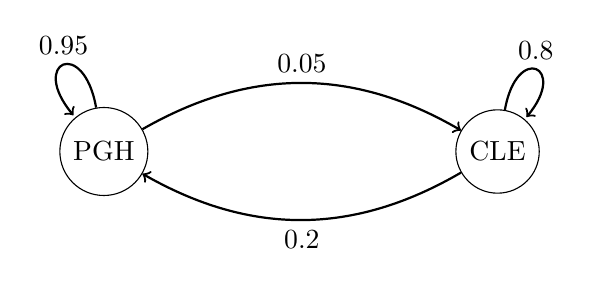
\begin{tikzpicture}
        \node (pgh) [circle,draw] {PGH}
            edge [out=100,in=130,loop,thick] node[above]{0.95} ()
        ;
        \node (cle) [circle,draw] at (5,0) {CLE}
            edge [out=80,in=50,loop,thick] node[above]{0.8} ()
        ;
        \draw [->,thick] (pgh) to[bend left=30] node[above]{0.05} (cle);
        \draw [->,thick] (cle) to[bend left=30] node[below]{0.2} (pgh);
    \end{tikzpicture}
\end{center}
\begin{itemize}
    \item $
        u_0 =
        \begin{bmatrix}
            500,000\\
            500,000\\
        \end{bmatrix}
    $
    \item $Au_0 = u_1$.
    \item $Au_1 = u_2$, $A(Au_0) = u_2$, $A^2u_0 = u_2$, $A^ku_0 = u_k$, $(S\Lambda S^{-1})^ku_0 = u_k$, $S\Lambda^kS^{-1}u_0 = u_k$.
    \begin{align*}
        A &=
        \begin{bmatrix}
            0.95 & 0.20\\
            0.05 & 0.80\\
        \end{bmatrix}&
        u_k &=
        \begin{bmatrix}
            \text{PGH}\\
            \text{CLE}\\
        \end{bmatrix}
    \end{align*}
    \item $A$ is a \textbf{Markov matrix}, where all columns and rows add to 1.
    \item $
        Au_0 =
        \begin{bmatrix}
            0.95 & 0.20\\
            0.05 & 0.80\\
        \end{bmatrix}
        \begin{bmatrix}
            500,000\\
            500,000\\
        \end{bmatrix}
        = u_1
    $
    \begin{align*}
        |A-\lambda I| &=
        \begin{vmatrix}
            0.95-\lambda & 0.20\\
            0.05 & 0.80-\lambda\\
        \end{vmatrix}\\
        &= (0.95-\lambda)(0.8-\lambda)-(0.2)(0.05)\\
        &= (\lambda-1)(\lambda-0.75)
    \end{align*}
    \item $\lambda_1 = 1,\ \lambda_2 = 0.75$.
    \item $
        A-I =
        \begin{bmatrix}
            -0.05 & 0.2\\
            0.05 & -0.2\\
        \end{bmatrix}
        \Rightarrow
        x =
        \begin{bmatrix}
            4\\
            1\\
        \end{bmatrix}
    $
    \item $
        A-0.75I =
        \begin{bmatrix}
            0.2 & 0.2\\
            0.05 & 0.05\\
        \end{bmatrix}
        \Rightarrow
        x =
        \begin{bmatrix}
            -1\\
            1\\
        \end{bmatrix}
    $
    \begin{align*}
        A^ku_0 &= \frac{1}{5}
        \begin{bmatrix}
            4 & -1\\
            1 & 1\\
        \end{bmatrix}
        \begin{bmatrix}
            1 & 0\\
            0 & 0.75\\
        \end{bmatrix}^k
        \begin{bmatrix}
            1 & 1\\
            -1 & 4\\
        \end{bmatrix}
        \begin{bmatrix}
            500,000\\
            500,000\\
        \end{bmatrix}\\
        &=
        \begin{bmatrix}
            4 & -1\\
            1 & 1\\
        \end{bmatrix}
        \begin{bmatrix}
            1 & 0\\
            0 & 0.75^k\\
        \end{bmatrix}
        \begin{bmatrix}
            200,000\\
            300,000\\
        \end{bmatrix}\\
        &=
        \begin{bmatrix}
            4\\
            1\\
        \end{bmatrix}
        (200,000) +
        \begin{bmatrix}
            -1\\
            1\\
        \end{bmatrix}
        (0.75)^k(300,000)
    \end{align*}
    \item $
        \begin{bmatrix}
            800,000\\
            200,000\\
        \end{bmatrix}
    $ is the steady-state vector.
    \item $
        \begin{bmatrix}
            -(0.75)^k(300,000)\\
            (0.75)^k(300,000)\\
        \end{bmatrix}
    $ is the dynamically changing vector.
    \item $
        \lim_{k\to\infty} A^ku_0 =
        \begin{bmatrix}
            800,000\\
            200,000\\
        \end{bmatrix}
        =
        \begin{bmatrix}
            \text{PGH}\\
            \text{CLE}\\
        \end{bmatrix}
    $
\end{itemize}


\subsection*{Explicit Formula for the Fibonacci Sequence}
\begin{itemize}
    \item \marginnote{2/4:}1, 1, 2, 3, 5, 8, \dots
    \item Recursively defined formula: $F_n$$^[$\footnote{The $n$-th Fibonacci number.}$^]$$=F_{n-1}+F_{n-2}$.
    \begin{align*}
        F_n &= F_{n-1}+F_{n-2}\\
        F_{n-1} &= F_{n-1}\\
        \begin{bmatrix}
            F_n\\
            F_{n-1}\\
        \end{bmatrix}
        &=
        \begin{bmatrix}
            1 & 1\\
            1 & 0\\
        \end{bmatrix}
        \begin{bmatrix}
            F_{n-1}\\
            F_{n-2}\\
        \end{bmatrix}
    \end{align*}
    \item $u_n = A^nu_0 = S\Lambda^nS^{-1}u_0$.
    \begin{align*}
        0 &= |A-\lambda I|\\
        &=
        \begin{vmatrix}
            1-\lambda & 1\\
            1 & -\lambda\\
        \end{vmatrix}\\
        &= -\lambda(1-\lambda)-1\\
        &= \lambda^2-\lambda-1
    \end{align*}
    \item $\lambda = \frac{1\pm\sqrt{5}}{2}$$^[$\footnote{This is the Golden ratio!}$^]$.
    \item $\lambda_1 = \frac{1+\sqrt{5}}{2}$.
    \begin{align*}
        N(A-\lambda_1I) &= N\left(
        \begin{bmatrix}
            1-\frac{1+\sqrt{5}}{2} & 1\\
            1 & -\frac{1+\sqrt{5}}{2}\\
        \end{bmatrix}
        \right)\\
        &= N\left(
        \begin{bmatrix}
            \frac{1-\sqrt{5}}{2} & 1\\
            1 & \frac{-1-\sqrt{5}}{2}\\
        \end{bmatrix}
        \right)\\
    \end{align*}
    \item $
        \begin{bmatrix}
            \frac{1-\sqrt{5}}{2} & 1\\
            1 & \frac{-1-\sqrt{5}}{2}\\
        \end{bmatrix}
        \begin{bmatrix}
            x_1\\
            x_2\\
        \end{bmatrix}
        =
        \begin{bmatrix}
            0\\
            0\\
        \end{bmatrix}
    $
    \item Let $x_2=1$.
    \begin{align*}
        \frac{1-\sqrt{5}}{2}x_1+1 &= 0\\
        \frac{1-\sqrt{5}}{2}x_1 &= -\frac{2}{2}\\
        x_1 &= \frac{-2}{1-\sqrt{5}}\times \frac{1+\sqrt{5}}{1+\sqrt{5}}\\
        &= \frac{-2-2\sqrt{5}}{-4}\\
        &= \frac{1+\sqrt{5}}{2}
    \end{align*}
    \item $
        s_1 =
        \begin{bmatrix}
            \frac{1+\sqrt{5}}{2}\\
            1\\
        \end{bmatrix}
    $, $
        s_2 =
        \begin{bmatrix}
            \frac{1-\sqrt{5}}{2}\\
            1\\
        \end{bmatrix}
    $.
    \item $
        \begin{bmatrix}
            1 & 1\\
            1 & 0\\
        \end{bmatrix}
        =
        \begin{bmatrix}
            \frac{1+\sqrt{5}}{2} & \frac{1-\sqrt{5}}{2}\\
            1 & 1\\
        \end{bmatrix}
        \begin{bmatrix}
            \frac{1+\sqrt{5}}{2} & 0\\
            0 & \frac{1-\sqrt{5}}{2}\\
        \end{bmatrix}
        S^{-1}
    $
    \item $
        S^{-1}
        = \frac{1}{|S|}C_S^\T
        = \frac{1}{\sqrt{5}}
        \begin{bmatrix}
            1 & \frac{-1+\sqrt{5}}{2}\\
            -1 & \frac{1+\sqrt{5}}{2}\\
        \end{bmatrix}
    $
    \item $u_k = A^ku_0 = S\Lambda^kS^{-1}u_0$.
    \begin{align*}
        S^{-1}u_0 &= \frac{1}{\sqrt{5}}
        \begin{bmatrix}
            1 & \frac{-1+\sqrt{5}}{2}\\
            -1 & \frac{1+\sqrt{5}}{2}\\
        \end{bmatrix}
        \begin{bmatrix}
            1\\
            1\\
        \end{bmatrix}\\
        &= \frac{1}{\sqrt{5}}
        \begin{bmatrix}
            \frac{1+\sqrt{5}}{2}\\
            \frac{-1+\sqrt{5}}{2}\\
        \end{bmatrix}\\
        &=
        \begin{bmatrix}
            \frac{1+\sqrt{5}}{2\sqrt{5}}\\
            \frac{-1+\sqrt{5}}{2\sqrt{5}}\\
        \end{bmatrix}\\
        &=
        \begin{bmatrix}
            \frac{5+\sqrt{5}}{10}\\
            \frac{5-\sqrt{5}}{10}\\
        \end{bmatrix}
    \end{align*}
    \item $
        u_k =
        \begin{bmatrix}
            \frac{1+\sqrt{5}}{2}\\
            1\\
        \end{bmatrix}
        \left( \frac{1+\sqrt{5}}{2} \right)^k\left( \frac{5+\sqrt{5}}{10} \right)+
        \begin{bmatrix}
            \frac{1-\sqrt{5}}{2}\\
            1\\
        \end{bmatrix}
        \left( \frac{1-\sqrt{5}}{2} \right)^k\left( \frac{5-\sqrt{5}}{10} \right)
    $
\end{itemize}



\section*{Systems of First-Order Ordinary Differential Equations}
\begin{itemize}
    \item \marginnote{2/11:}Let $f(x)=y$ and $a,c,K\in\mathbb{F}$.
    \begin{align*}
        \dd[y]{x} &= ay\\
        \frac{1}{y}\dd[y]{x} &= a\\
        \frac{1}{y}\dd[y]{x}\, \dx &= a\, \dx\\
        \frac{1}{y}\, \dy &= a\, \dx\\
        \int \frac{1}{y}\, \dy &= \int a\, \dx\\
        \ln y &= ax+c\\
        y &= \e^{ax+c}\\
        &= \e^{ax}\text{e}^c\\
        &= K\e^{ax}
    \end{align*}
    \item Let $\dd[y]{x}=y'$.
    \begin{itemize}
        \item $y_1' = a_{11}y_1+a_{12}y_2+\cdots+a_{1n}y_n$.
        \item $y_2' = a_{21}y_1+a_{22}y_2+\cdots+a_{2n}y_n$.
        \item $\vdots$
        \item $y_n' = a_{n1}y_1+a_{n2}y_2+\cdots+a_{nn}y_n$.
    \end{itemize}
    \item This is a \textbf{square system} of equations.
    \item Rewrite as $y' = Ay$.
    \begin{equation*}
        \begin{bmatrix}
            y_1'\\
            y_2'\\
            \vdots\\
            y_n'\\
        \end{bmatrix}
        =
        \begin{bmatrix}
            a_{11} & a_{12} & \cdots & a_{1n}\\
            a_{21} & a_{22} & \cdots & a_{2n}\\
            \vdots &        & \ddots &       \\
            a_{n1} & a_{n2} & \cdots & a_{nn}\\
        \end{bmatrix}
        \begin{bmatrix}
            y_1\\
            y_2\\
            \vdots\\
            y_n\\
        \end{bmatrix}
    \end{equation*}
    \item Solve the following system of differential equations.
    \begin{align*}
        y_1' &= 3y_1\\
        y_2' &= -2y_2\\
        y_3' &= 5y_3
    \end{align*}
    \begin{equation*}
        \begin{bmatrix}
            y_1'\\
            y_2'\\
            y_3'\\
        \end{bmatrix}
        =
        \begin{bmatrix}
            3 & 0 & 0\\
            0 & -2 & 0\\
            0 & 0 & 5\\
        \end{bmatrix}
        \begin{bmatrix}
            y_1\\
            y_2\\
            y_3\\
        \end{bmatrix}
    \end{equation*}
    \begin{itemize}
        \item General Solution:
    \end{itemize}
    \begin{align*}
        y_1 &= k_1\e^{3x}\\
        y_2 &= k_2\e^{-2x}\\
        y_3 &= k_3\e^{5x}
    \end{align*}
    \begin{itemize}
        \item Particular Solution (where $y_1(0)=2$, $y_2(0)=-1$, and $y_3(0)=7$ are the initial conditions):
    \end{itemize}
    \begin{align*}
        y_1 &= 2\e^{3x}\\
        y_2 &= -\e^{-2x}\\
        y_3 &= 7\e^{5x}
    \end{align*}
    \item Consider a different system. Remember throughout that we are solving for $y$.
    \begin{align*}
        y_1' &= y_1+y_2\\
        y_2' &= 4y_1-2y_2
    \end{align*}
    \begin{itemize}
        \item The previous system was so easy to solve because the matrix was diagonal. This one (as follows) will not be. Therefore, we should diagonalize it.
    \end{itemize}
    \begin{equation*}
        \begin{bmatrix}
            y_1'\\
            y_2'\\
        \end{bmatrix}
        =
        \begin{bmatrix}
            1 & 1\\
            4 & -2\\
        \end{bmatrix}
        \begin{bmatrix}
            y_1\\
            y_2\\
        \end{bmatrix}
    \end{equation*}
    \begin{itemize}
        \item Start with $y'=Ay$.
        \item Substitute $y=Su$.
        \begin{itemize}
            \item Note that $y=Su\Rightarrow y'=Su'$$^[$\footnote{Think about differentiating both sides: $y\rightarrow y'$ is obvious, $S$ will be unchanged because it's just coefficients, and the functions of $u$ will be differentiated.}$^]$.
            \item If we can find $u'$ in terms of a diagonal matrix and $u$, we can solve for $y$.
        \end{itemize}
        \begin{center}
            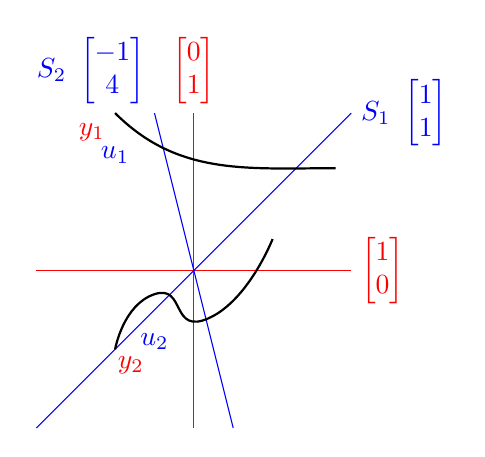
\begin{tikzpicture}
                \draw [red] (-2,0) -- (2,0) node[right]{
                    $
                        \begin{bmatrix}
                            1\\
                            0\\
                        \end{bmatrix}
                    $
                };
                \draw [red] (0,-2) -- (0,2) node[above]{
                    $
                        \begin{bmatrix}
                            0\\
                            1\\
                        \end{bmatrix}
                    $
                };

                \draw [blue] (-0.5,2) node[above left]{
                    $
                        S_2\
                        \begin{bmatrix}
                            -1\\
                            4\\
                        \end{bmatrix}
                    $
                } -- (0.5,-2);
                \draw [blue] (-2,-2) -- (2,2) node[right]{
                    $
                        S_1\
                        \begin{bmatrix}
                            1\\
                            1\\
                        \end{bmatrix}
                    $
                };

                \draw [thick] (-1,2) node[below left]{
                    $\color{red}y_1$
                } node[below=3mm]{
                    $\color{blue}u_1$
                } to[out=-45,in=180] (1.8,1.3);
                \draw [thick] plot[smooth,tension=1.2] coordinates{
                    (-1,-1) (-0.5,-0.3) (0.2,-0.6) (1,0.4)
                };
                \node at (-0.8,-1.2) {
                    $\color{red}y_2$
                };
                \node at (-0.5,-0.9) {
                    $\color{blue}u_2$
                };
            \end{tikzpicture}
        \end{center}
        \item We seek to find a new basis $S$ such that the matrix scaling $u$ will be diagonal.
    \end{itemize}
    \begin{align*}
        Su' &= Ay\\
        Su' &= ASu\\
        u' &= S^{-1}ASu\\
        u' &= \Lambda u
    \end{align*}
    \begin{itemize}
        \item The last substitution above is legal because if $A=S\Lambda S^{-1}$, then $\Lambda=S^{-1}AS$.
    \end{itemize}
    \begin{align*}
        0 &=
        \begin{vmatrix}
            1-\lambda & 1\\
            4 & -2-\lambda\\
        \end{vmatrix}\\
        &= (1-\lambda)(-2-\lambda)-4\\
        &= -2-\lambda+2\lambda+\lambda^2-4\\
        &= \lambda^2+\lambda-6\\
        &= (\lambda-2)(\lambda+3)
    \end{align*}
    \begin{align*}
        \lambda_1 &= 2&
        \lambda_2 &= -3
    \end{align*}
    \begin{itemize}
        \item $
            A-2I=
            \begin{bmatrix}
                -1 & 1\\
                4 & -4\\
            \end{bmatrix}
            \begin{bmatrix}
                1\\
                1\\
            \end{bmatrix}
            =
            \begin{bmatrix}
                0\\
                0\\
            \end{bmatrix}
        $
        \item $
            A+3I=
            \begin{bmatrix}
                4 & 1\\
                4 & 1\\
            \end{bmatrix}
            \begin{bmatrix}
                -1\\
                4\\
            \end{bmatrix}
            =
            \begin{bmatrix}
                0\\
                0\\
            \end{bmatrix}
        $
    \end{itemize}
    \begin{align*}
        u' &= \Lambda u\\
        \begin{bmatrix}
            u_1'\\
            u_2'\\
        \end{bmatrix}
        &=
        \begin{bmatrix}
            2 & 0\\
            0 & -3\\
        \end{bmatrix}
        \begin{bmatrix}
            u_1\\
            u_2\\
        \end{bmatrix}
    \end{align*}
    \begin{align*}
        u_1 &= k_1\e^{2x}\\
        u_2 &= k_2\e^{-3x}
    \end{align*}
    \begin{align*}
        y &= Su\\
        \begin{bmatrix}
            y_1\\
            y_2\\
        \end{bmatrix}
        &=
        \begin{bmatrix}
            1 & -1\\
            1 & 4\\
        \end{bmatrix}
        \begin{bmatrix}
            k_1\e^{2x}\\
            k_2\e^{-3x}\\
        \end{bmatrix}
    \end{align*}
    \begin{align*}
        y_1 &= k_1\e^{2x}-k_2\e^{-3x}\\
        y_2 &= k_1\e^{2x}+4k_2\e^{-3x}
    \end{align*}
    \item \marginnote{2/12:}Initial conditions: $y_1(0)=1$ and $y_2(0)=6$.
    \begin{itemize}
        \item Use augmented matrices to solve a system of equations.
    \end{itemize}
    \begin{equation*}
        \begin{amatrix}{2}
            1 & -1 & 1\\
            1 & 4 & 6\\
        \end{amatrix}
        \rightarrow
        \begin{amatrix}{2}
            1 & 0 & 2\\
            0 & 1 & 1\\
        \end{amatrix}
    \end{equation*}
    \item Particular solution:
    \begin{align*}
        y_1 &= 2\e^{2x}-\e^{-3x}\\
        y_2 &= 2\e^{2x}+4\e^{-3x}
    \end{align*}
\end{itemize}


\subsection*{Matrix Exponentiation}
\begin{itemize}
    \item $\e^A$ is a matrix defined as the infinite sum of a power series.
    \item $f(t) = \e^t$.
\end{itemize}
\begin{tchart}{1.6}{Differential Equations}{Power Series}
    $f'(t)=f(t)$ & $f(t)=1+t+\frac{t^2}{2}+\frac{t^3}{3!}+\cdots$\\
    $f(0)=1$ & $\frac{\text{d}}{\text{d}t}(t)=1$, $\frac{\text{d}}{\text{d}t}\left( \frac{t^2}{2} \right)=t$, \dots\\
    & $f(t)=\sum_{n=0}^\infty \frac{t^n}{n!}$
\end{tchart}
\begin{itemize}
    \item $f(t)=\e^{at}$.
\end{itemize}
\begin{tchart}{1.5}{Differential Equations}{Power Series}
    $f'(t)=af(t)$ & $f(t)=\sum_{n=0}^\infty \frac{a^nt^n}{n!}$\\
    $f(0)=1$ &\\
\end{tchart}
\begin{itemize}
    \item $F(t)=\e^{At}$.
    \begin{itemize}
        \item A matrix-valued function.
        \item Ex. $
            F(\theta) =
            \begin{bmatrix}
                \cos(\theta) & -\sin(\theta)\\
                \sin(\theta) & \cos(\theta)\\
            \end{bmatrix}
        $
        \item $F(\theta)A$ rotates points (arrows) of $A$ by $\theta$.
    \end{itemize}
\end{itemize}
\begin{tchart}{1.5}{Differential Equations}{Power Series}
    $F'(t)=A\e^{At}$ & $F(t)=I+At+\frac{A^2t^2}{2!}+\frac{A^3t^3}{3!}+\cdots$\\
    $F(0)=I$ & $F(t)=\sum_{n=0}^\infty \frac{A^nt^n}{n!}$\\
\end{tchart}


\subsection*{Diagonalization of e\textsuperscript{\emph{At}}}
\begin{itemize}
    \item Find an alternate form for $\e^{At}$ by manipulating its power series definition:
    \begin{align*}
        \e^{At} &= \sum_{n=0}^\infty \frac{A^nt^n}{n!}\\
        &= \sum_{n=0}^\infty \frac{S\Lambda^nS^{-1}t^n}{n!}\\
        &= \sum_{n=0}^\infty S\left( \frac{\Lambda^nt^n}{n!} \right)S^{-1}\\
        &= S\left( {\color{grx}\sum_{n=0}^\infty \frac{t^n}{n!}\Lambda^n} \right)S^{-1}\\
        &= S\left( \sum_{n=0}^\infty \frac{t^n}{n!}
        \begin{bmatrix}
            \lambda_1 &  & \\
             & \ddots & \\
             &  & \lambda_k\\
        \end{bmatrix}^n
        \right)S^{-1}\\
        &= S\left( \sum_{n=0}^\infty \frac{t^n}{n!}
        \begin{bmatrix}
            \lambda_1^n &  & \\
             & \ddots & \\
             &  & \lambda_k^n\\
        \end{bmatrix}
        \right)S^{-1}\\
        &= S\left( \sum_{n=0}^\infty
        \begin{bmatrix}
            \frac{t^n}{n!}\lambda_1^n &  & \\
             & \ddots & \\
             &  & \frac{t^n}{n!}\lambda_k^n\\
        \end{bmatrix}
        \right)S^{-1}\\
        &= S\left( \sum_{n=0}^\infty
        \begin{bmatrix}
            \frac{\lambda_1^nt^n}{n!} &  & \\
             & \ddots & \\
             &  & \frac{\lambda_k^nt^n}{n!}\\
        \end{bmatrix}
        \right)S^{-1}\\
        \marginnote{2/13:}&= S
        \begin{bmatrix}
            \sum_{n=0}^\infty \frac{\lambda_1^nt^n}{n!} &  & \\
             & \ddots & \\
             &  & \sum_{n=0}^\infty \frac{\lambda_k^nt^n}{n!}\\
        \end{bmatrix}
        S^{-1}\\
        &= S
        \begin{bmatrix}
            \e^{\lambda_1t} &  & \\
             & \ddots & \\
             &  & \e^{\lambda_kt}\\
        \end{bmatrix}
        S^{-1}\\
        &= S{\color{grx}\e^{\Lambda t}}S^{-1}\\
        &= F(t)
    \end{align*}
    \item Prove, using the above result, that $F'(t)$ can be defined in terms of $F(t)$:
    \begin{align*}
        F(t) &= \e^{At}\\
        &= S
        \begin{bmatrix}
            \e^{\lambda_1t} &  & \\
             & \ddots & \\
             &  & \e^{\lambda_kt}\\
        \end{bmatrix}
        S^{-1}
    \end{align*}
    \begin{align*}
        F'(t) &= \dd{t}\left( S
        \begin{bmatrix}
            \e^{\lambda_1t} &  & \\
             & \ddots & \\
             &  & \e^{\lambda_kt}\\
        \end{bmatrix}
        S^{-1} \right)\\
        &= S\dd{t}\left(
        \begin{bmatrix}
            \e^{\lambda_1t} &  & \\
             & \ddots & \\
             &  & \e^{\lambda_kt}\\
        \end{bmatrix}
        \right)S^{-1}\\
        &= S
        \begin{bmatrix}
            \dd{t}\e^{\lambda_1t} &  & \\
             & \ddots & \\
             &  & \dd{t}\e^{\lambda_kt}\\
        \end{bmatrix}
        S^{-1}\\
        &= S
        \begin{bmatrix}
            \lambda_1\e^{\lambda_1t} &  & \\
             & \ddots & \\
             &  & \lambda_k\e^{\lambda_kt}\\
        \end{bmatrix}
        S^{-1}\\
        &= S
        \begin{bmatrix}
            \lambda_1 &  & \\
             & \ddots & \\
             &  & \lambda_k\\
        \end{bmatrix}
        \begin{bmatrix}
            \e^{\lambda_1t} &  & \\
             & \ddots & \\
             &  & \e^{\lambda_kt}\\
        \end{bmatrix}
        S^{-1}\\
        &= S
        \begin{bmatrix}
            \lambda_1 &  & \\
             & \ddots & \\
             &  & \lambda_k\\
        \end{bmatrix}
        I_k
        \begin{bmatrix}
            \e^{\lambda_1t} &  & \\
             & \ddots & \\
             &  & \e^{\lambda_kt}\\
        \end{bmatrix}
        S^{-1}\\
        &= {\color{red}S
        \begin{bmatrix}
            \lambda_1 &  & \\
             & \ddots & \\
             &  & \lambda_k\\
        \end{bmatrix}
        S^{-1}}{\color{blue}S
        \begin{bmatrix}
            \e^{\lambda_1t} &  & \\
             & \ddots & \\
             &  & \e^{\lambda_kt}\\
        \end{bmatrix}
        S^{-1}}\\
        &= {\color{red}A}{\color{blue}F(t)}\\
        &= A\e^{At}
    \end{align*}
    \item In other words, $y'(t)=Ay(t)$ and $y(0)=y_0$. The solution is $y=\e^{At}y_0$.
    \item Example:
    \begin{align*}
        y'_1 &= 5y_1+y_2& y_1(0) &= -3\\
        y'_2 &= -2y_1+2y_2& y_2(0) &= 8
    \end{align*}
    \begin{align*}
        y(t) &= \e^{At}y(0)\\
        &= S\e^{\Lambda t}S^{-1}y(0)
    \end{align*}
    \begin{align*}
        0 &= |A-\lambda I|\\
        &=
        \begin{vmatrix}
            5-\lambda & 1\\
            -2 & 2-\lambda\\
        \end{vmatrix}\\
        &= (\lambda-3)(\lambda-4)
    \end{align*}
    \begin{itemize}
        \item $
            A-3I =
            \begin{bmatrix}
                2 & 1\\
                -2 & -1\\
            \end{bmatrix}
        $
        \item $
            N(A-3I) = \left\{
            \begin{bmatrix}
                1\\
                -2\\
            \end{bmatrix}
            \right\}
        $
        \item $
            A-4I =
            \begin{bmatrix}
                1 & 1\\
                -2 & -2\\
            \end{bmatrix}
        $
        \item $
            N(A-4I) = \left\{
            \begin{bmatrix}
                -1\\
                1\\
            \end{bmatrix}
            \right\}
        $
    \end{itemize}
    \begin{align*}
        y(t) &= S\e^{\Lambda t}S^{-1}y(0)\\
        &=
        \begin{bmatrix}
            1 & -1\\
            -2 & 1\\
        \end{bmatrix}
        \begin{bmatrix}
            \e^{3t} & 0\\
            0 & \e^{4t}\\
        \end{bmatrix}
        \begin{bmatrix}
            -1 & -1\\
            -2 & -1\\
        \end{bmatrix}
        \begin{bmatrix}
            -3\\
            8\\
        \end{bmatrix}\\
        &=
        \begin{bmatrix}
            \e^{3t} & -\e^{4t}\\
            -2\e^{3t} & \e^{4t}\\
        \end{bmatrix}
        \begin{bmatrix}
            -1 & -1\\
            -2 & -1\\
        \end{bmatrix}
        \begin{bmatrix}
            -3\\
            8\\
        \end{bmatrix}\\
        &=
        \begin{bmatrix}
            -\e^{3t}+2\e^{4t} & -\e^{3t}+\e^{4t}\\
            2\e^{3t}-2\e^{4t} & 2\e^{3t}-\e^{4t}\\
        \end{bmatrix}
        \begin{bmatrix}
            -3\\
            8\\
        \end{bmatrix}\\
        &=
        \begin{bmatrix}
            3\e^{3t}-6\e^{4t}-8\e^{3t}+8\e^{4t}\\
            -6\e^{3t}+6\e^{4t}+16\e^{3t}-8\e^{4t}\\
        \end{bmatrix}\\
        &=
        \begin{bmatrix}
            -5\e^{3t}+2\e^{4t}\\
            10\e^{3t}-2\e^{4t}\\
        \end{bmatrix}\\
        &=
        \begin{bmatrix}
            y_1(t)\\
            y_2(t)\\
        \end{bmatrix}
    \end{align*}
\end{itemize}



\section*{Orthonormally Diagonalizable Matrices}
\begin{itemize}
    \item \marginnote{2/19:}$A=Q\Lambda Q^\T$.
    \begin{itemize}
        \item Eigenvectors are orthonormal.
    \end{itemize}
    \item $A^\T = \left( Q\Lambda Q^\T \right)^\T = Q^{\T\T}\Lambda^\T Q^\T = Q\Lambda Q^\T = A$.
    \item Prove that the symmetric matrices are exactly those that are orthonormally diagonalizable.
    \begin{itemize}
        \item Let $A = A^\T$.
        \begin{equation}\label{eqn:ortho1}
            Ax_1 = \lambda_1x_1
        \end{equation}
        \begin{equation}\label{eqn:ortho2}
            Ax_2 = \lambda_2x_2
        \end{equation}
        \item Multiply Equation \ref{eqn:ortho1} by $x_2^\T$ from Equation \ref{eqn:ortho2}.
        \begin{itemize}
            \item We have to relate the two equations.
            \item Later, we transpose, because we have to specifically target the properties of symmetric matrices.
        \end{itemize}
        \begin{align*}
            \lambda_1x_2^\T x_1 &= x_2^\T Ax_1\\
            &= (x_2^\T A)x_1\\
            &= \left( A^\T x_2 \right)^\T x_1\\
            &= \left( A x_2 \right)^\T x_1\\
            \lambda_1x_2^\T x_1 &= \lambda_2x_2^T x_1\\
            \lambda_1x_2^\T x_1-\lambda_2x_2^T x_1 &= 0\\
            x_2^\T x_1(\lambda_1-\lambda_2) &= 0
        \end{align*}
        \item The last line above implies that $x_2^\T x_1 = 0$ iff $\lambda_1\neq\lambda_2$.
    \end{itemize}
    \item The only matrices that we can guarantee will never have complex eigenvalues are symmetric matrices.
    \item On complex numbers/vectors:
    \begin{itemize}
        \item $z=a+bi$ and $\bar{z}=a-bi$, where $a,b\in\R$, $i=\sqrt{-1}$.
        \item $z\bar{z} = a^2+b^2$.
        \item $
            x =
            \begin{bmatrix}
                a_1+b_1i\\
                \vdots\\
                a_n+b_ni\\
            \end{bmatrix}
        $ and $
            \bar{x} =
            \begin{bmatrix}
                a_1-b_1i\\
                \vdots\\
                a_n-b_ni\\
            \end{bmatrix}
        $.
    \end{itemize}
    \item Prove that when $A = A^\T$, $\lambda_n\in\R$.
    \begin{itemize}
        \item Let $A = A^\T$, $A\in\R^n$.
        \begin{equation}\label{eqn:ortho3}
            Ax = \lambda x
        \end{equation}
        \begin{equation*}
            \bar{A}\bar{x} = \bar{\lambda}\bar{x}
        \end{equation*}
        \item If $A\in\R^n$, then $A=\bar{A}$.
        \begin{align*}
            A\bar{x} &= \bar{\lambda}\bar{x}\\
            \left( A\bar{x} \right)^\T &= \left( \bar{\lambda}\bar{x} \right)^\T\\
            \bar{x}^\T A^\T &= \bar{\lambda}\bar{x}^\T\\
            \bar{x}^\T A &= \bar{\lambda}\bar{x}^\T\stepcounter{equation}\tag{\theequation}\label{eqn:ortho4}\\
        \end{align*}
        \item Multiply Equation \ref{eqn:ortho3} by $\bar{x}^\T$ from the left.
        \begin{itemize}
            \item ${\color{blue}\bar{x}^\T Ax} = {\color{red}\lambda\bar{x}^\T x}$.
        \end{itemize}
        \item Multiply Equation \ref{eqn:ortho4} by $x$ from the right.
        \begin{itemize}
            \item ${\color{blue}\bar{x}^\T Ax} = {\color{grx}\bar{\lambda}\bar{x}^\T x}$.
        \end{itemize}
        \item ${\color{red}\lambda\bar{x}^\T x} = {\color{grx}\bar{\lambda}\bar{x}^\T x} \Rightarrow \lambda = \bar{\lambda} \Rightarrow \lambda\in\R$.
    \end{itemize}
\end{itemize}



\subsection*{Spectral Decomposition}
\marginnote{2/20:}\begin{equation*}
    A =
    \begin{bmatrix}
        2 & 1 & 1\\
        1 & 2 & 1\\
        1 & 1 & 2\\
    \end{bmatrix}
\end{equation*}
\begin{itemize}
    \item $\lambda_1 = 4,\ \lambda_2=\lambda_3=1$.
    \item $
        x_1 =
        \begin{bmatrix}
            1\\
            1\\
            1\\
        \end{bmatrix}
    $, $
        x_2 =
        \begin{bmatrix}
            -1\\
            0\\
            1\\
        \end{bmatrix}
    $, $
        x_3 =
        \begin{bmatrix}
            -1\\
            1\\
            0\\
        \end{bmatrix}
    $.
    \begin{itemize}
        \item $x_1^\T x_2 = 0$, $x_1^\T x_3 = 0$, $x_2^\T x_3 = -1$.
    \end{itemize}
    \item Orthogonalize by Gram-Schmidt, inspection, put the vectors in a matrix and find the null space (the null vector will be orthogonal by the fundamental theorem).
    \item $
        x_3' =
        \begin{bmatrix}
            -1\\
            2\\
            -1\\
        \end{bmatrix}
    $.
    \begin{itemize}
        \item $x_3'$ is not scaled along its line by $A$, but it is scaled in the plane of $x_2$ and $x_3$ by $A$.
        \item $x_1^\T x_3' = 0$, $x_2^\T x_3' = 0$.
    \end{itemize}
    \item $
        q_1 = \frac{1}{\sqrt{3}}
        \begin{bmatrix}
            1\\
            1\\
            1\\
        \end{bmatrix}
    $, $
        q_2 = \frac{1}{\sqrt{2}}
        \begin{bmatrix}
            -1\\
            0\\
            1\\
        \end{bmatrix}
    $, $
        q_3 = \frac{1}{\sqrt{6}}
        \begin{bmatrix}
            -1\\
            2\\
            -1\\
        \end{bmatrix}
    $.
    \begin{align*}
        A &= Q\Lambda Q^\T\\
        &=
        \begin{bmatrix}
            | &  & |\\
            q_1 & \cdots & q_n\\
            | &  & |\\
        \end{bmatrix}
        \begin{bmatrix}
            \lambda_1 &  & \\
             & \ddots & \\
             &  & \lambda_n\\
        \end{bmatrix}
        \begin{bmatrix}
            \text{---} & q_1^\T & \text{---}\\
             & \vdots & \\
            \text{---} & q_n^\T & \text{---}\\
        \end{bmatrix}\\
        &=
        \begin{bmatrix}
            | &  & |\\
            q_1\lambda_1 & \cdots & q_n\lambda_n\\
            | &  & |\\
        \end{bmatrix}
        \begin{bmatrix}
            \text{---} & q_1^\T & \text{---}\\
             & \vdots & \\
            \text{---} & q_n^\T & \text{---}\\
        \end{bmatrix}\\
        &= \lambda_1q_1q_1^\T+\cdots+\lambda_nq_nq_n^\T
    \end{align*}
    \renewcommand{\arraystretch}{1.6}
    \item $
        q_1q_1^\T =
        \begin{bmatrix}
            \frac{1}{\sqrt{3}}\\
            \frac{1}{\sqrt{3}}\\
            \frac{1}{\sqrt{3}}\\
        \end{bmatrix}
        \begin{bmatrix}
            \frac{1}{\sqrt{3}} & \frac{1}{\sqrt{3}} & \frac{1}{\sqrt{3}}\\
        \end{bmatrix}
        =
        \begin{bmatrix}
            \frac{1}{3} & \frac{1}{3} & \frac{1}{3}\\
            \frac{1}{3} & \frac{1}{3} & \frac{1}{3}\\
            \frac{1}{3} & \frac{1}{3} & \frac{1}{3}\\
        \end{bmatrix}
    $
    \item $
        q_2q_2^\T =
        \begin{bmatrix}
            -\frac{1}{\sqrt{2}}\\
            0\\
            \frac{1}{\sqrt{2}}\\
        \end{bmatrix}
        \begin{bmatrix}
            -\frac{1}{\sqrt{2}} & 0 & \frac{1}{\sqrt{2}}\\
        \end{bmatrix}
        =
        \begin{bmatrix}
            \frac{1}{2} & 0 & -\frac{1}{2}\\
            0 & 0 & 0\\
            -\frac{1}{2} & 0 & \frac{1}{2}\\
        \end{bmatrix}
    $
    \item $
        q_3q_3^\T =
        \begin{bmatrix}
            -\frac{1}{\sqrt{6}}\\
            \frac{2}{\sqrt{6}}\\
            -\frac{1}{\sqrt{6}}\\
        \end{bmatrix}
        \begin{bmatrix}
            -\frac{1}{\sqrt{6}} & \frac{2}{\sqrt{6}} & -\frac{1}{\sqrt{6}}\\
        \end{bmatrix}
        =
        \begin{bmatrix}
            \frac{1}{6} & -\frac{1}{3} & \frac{1}{6}\\
            -\frac{1}{3} & \frac{2}{3} & -\frac{1}{3}\\
            \frac{1}{6} & -\frac{1}{3} & \frac{1}{6}\\
        \end{bmatrix}
    $
    \item $
        A = 4
        \begin{bmatrix}
            \frac{1}{3} & \frac{1}{3} & \frac{1}{3}\\
            \frac{1}{3} & \frac{1}{3} & \frac{1}{3}\\
            \frac{1}{3} & \frac{1}{3} & \frac{1}{3}\\
        \end{bmatrix}
        +
        \begin{bmatrix}
            \frac{1}{2} & 0 & -\frac{1}{2}\\
            0 & 0 & 0\\
            -\frac{1}{2} & 0 & \frac{1}{2}\\
        \end{bmatrix}
        +
        \begin{bmatrix}
            \frac{1}{6} & -\frac{1}{3} & \frac{1}{6}\\
            -\frac{1}{3} & \frac{2}{3} & -\frac{1}{3}\\
            \frac{1}{6} & -\frac{1}{3} & \frac{1}{6}\\
        \end{bmatrix}
    $
    \item $
        A = 4
        \begin{bmatrix}
            \frac{1}{3} & \frac{1}{3} & \frac{1}{3}\\
            \frac{1}{3} & \frac{1}{3} & \frac{1}{3}\\
            \frac{1}{3} & \frac{1}{3} & \frac{1}{3}\\
        \end{bmatrix}
        +
        \begin{bmatrix}
            \frac{2}{3} & -\frac{1}{3} & -\frac{1}{3}\\
            -\frac{1}{3} & \frac{2}{3} & -\frac{1}{3}\\
            -\frac{1}{3} & -\frac{1}{3} & \frac{2}{3}\\
        \end{bmatrix}
    $ is the spectral decomposition of $A$.
    \renewcommand{\arraystretch}{1}
\end{itemize}




\end{document}